\setcounter{secnumdepth}{1}
\section{Sphärische, elliptische und hyperbolische (nichteuklidische) Geometrie}
\setcounter{secnumdepth}{0}
Themen dieses Abschnitts: Inversion (Spiegelung) an Sphären, stereographische Projektion, Möbiusgruppen

\subsection{Inversion an Sphären}
\begin{defn*}
 Eine \emph{$(n-1)$-Sphäre} im $\real^n$ ist eine Menge der Form $\Gamma = \{ x \in \real^n : \| x - a \| = r \}$. $a \in \real^n$ ist der \emph{Mittelpunkt} und $r$ der \emph{Radius} der Sphäre.
 
 Eine $(m-1)$-Späre im $\real^n$ ist eine Menge $\Sigma$ der Form $\Sigma = \Gamma \cap A$, wobei $\Gamma$ eine $(n-1)$-Sphäre ist und $A$ ein $m$-dimensionaler affiner Unterraum des $\real^n$ mit $| \Gamma \cap A | \ge 2$.
\end{defn*}

\textbf{Es gilt:} Der Durchschnitt von zwei verschiedenen $(n-1)$-Sphären im $\real^n$ ist entweder $\emptyset$ oder ein Punkt oder eine $(n-2)$-Sphäre.

\begin{proof}
 Für die Schnittmenge gilt
 \[ \| x-a \|^2 = r^2 \wedge \| x-b \| = s^2. \]
 Es ist $\| x-a \|^2 = \angles{x-a,x-a}$, also gilt
 \begin{align*}
  \| x^2 \| - 2 \angles{a,x} + \| a \|^2 &= r^2 \quad \wedge  \tag{1} \\
  \| x^2 \| - 2 \angles{b,x} + \| b \|^2 &= s^2 \tag{2}
 \end{align*}
 Subtraktion $(1)-(2)$ liefert
 \[ 2 \angles{ b-a, x } + \| a \|^2 - \| b \|^2 = r^2 - s^2. \] 
 Das ist für $a \ne b$ die Gleichung einer Hyperebene (für $a=b$, $r \ne s$ nicht erfüllbar, also $\emptyset$).

 Die Gleichungen (1) und (2) sind äquivalent zu den Gleichungen (1) und (1)-(2), also dem Schnitt einer Hyperebene mit einer $(n-1)$-Sphäre.
\end{proof}

Betrachte zunächst die Einheitssphäre $\Gamma_0 = \{ x \in \real^n : \| x \| = 1 \}$. Die \emph{Inversion an der Einheitssphäre} ist die Abbildung $f$, die $x$ und $x'$ vertauscht, also
\[ \Phi_{\Gamma_0}(x) = f(x) = \frac{x}{\| x \|^2}. \]

Definiere $\hat{\real}^n = \real^n \cup \{ \infty \}$. $f(0) = \infty$, $f(\infty) = 0$.

Sei nun $\Gamma = \{ x \in \real^n | \| x-a \| = r \}$. Sei $g$ die Streckung bzw. Translation, die $\Gamma$ auf $\Gamma_0$ abbildet, also $g(x) = \frac{x-a}{r}$, $g^{-1}(x) = rx + a$.

Definiere $\Phi_\Gamma = g^{-1} \cdot \Phi_{\Gamma_0} \cdot g$, also 
\[ \Phi_\Gamma(x) = g^{-1} \left( \frac{1}{\| (x-a)/r \|^2} \cdot \frac{x-a}{r} \right) = \frac{r^2}{\|x-a\|^2}(x-a) + a \]
für $x \ne 0, \infty$. Es ist
\[ \Phi_\Gamma( 0 ) = \infty, \qquad \Phi_\Gamma( \infty ) = 0. \]
Für die Fixpunkte der Abbildung folgt
\[ \Phi_\Gamma(x) = x \Leftrightarrow x \in \Gamma, \]
und es gilt
\[ \Phi_\Gamma \circ \Phi_\Gamma = g^{-1} \Phi g g^{-1} \Phi g = g^{-1} \Phi^2 g = \id. \]

\subsection{Die stereographische Projektion}
\begin{defn*}
 Sei $\Gamma \subseteq \real^n$ eine $(n-1)$-Sphäre. Sei $x_0 \in \Gamma$ und $\Pi$ eine Hyperebene parallel zur Tangentialebene $\Pi_0$ an $x_0$, die im selben Halbraum wie $\Gamma$ liegt.

 Die \emph{stereographische Projektion von $x_0$ aus} auf $\Pi$ ist eine
 Abbildung  $\varphi: \Gamma \to \Pi \cup \{ \infty \}$.

 $\varphi(x)$ ist der Schnittpunkt der Geraden $x_0 x$ mit $\Pi$ für $x \ne
 x_0$, $\varphi(x_0) = \infty$.

 \begin{center}
   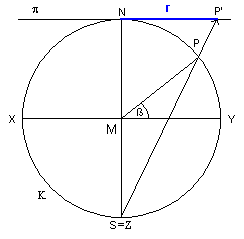
\includegraphics{img/stereo}
 \end{center}
 
 Das heißt, alle Punkte $x \in \Gamma$ werden auf den Punkt der Hyperebene
 abgebildet, an dem die Verbindungsgerade zwischen $x$ und $x_0$ die Ebene
 schneidet. Da für $x_0$ keine solche Gerade mit sich selbst  existiert,
 vereinbart man $\varphi(x_0) = \infty$.

 $\varphi$ ist offenbar bijektiv.
\end{defn*}

\subsection{Inversion (Spiegelung) an Hypersphären einer Sphäre}
Sei $\Gamma \subseteq \real^{n+1}$ eine $n$-Sphäre und $\Sigma \subseteq \Gamma$
eine $(n-1)$-Sphäre (\emph{Hypersphäre} in $\Gamma$). Dann ist $\Sigma = \Gamma
\cap H$ für eine Hyperebene $H$.

Falls $H$ durch den Mittelpunkt $a$ von $\Gamma$ geht, nennt man $\Sigma$ eine
\emph{Großhypersphäre}, anderenfalls eine
\emph{Kleinhypersphäre}.

Betrachte zum Beispiel die Einheitskugel in $\real^3$. Schnitte mit Ebenen
ergeben immer Kreise, dies sind die Hypersphären. Geht die Schnittebene durch 0,
ist es eine Großhypersphäre.

\begin{defn*}
 Die \emph{Inversion (Spiegelung) an der Hypersphäre $\Sigma$} ist für eine
 Kleinhypersphäre $\Sigma$ definiert durch $\Phi_\Sigma: \Gamma \to \Gamma$.
 
 Betrachte die Spitze $x_0$ des Tangentialkegels, der $\Gamma$ in $\Sigma$
 berührt. $\Phi_\Sigma$ vertauscht die beiden Schnittpunkte eines Strahls von
 $x_0$ durch einen Punkt aus $\Gamma \setminus \Sigma$ und bildet alle $x \in
 \Sigma$ auf sich ab.

 Betrachte zum Beispiel wieder die Einheitskugel im $\real^3$. An einen Kreis
 auf der Kugel kann man einen Tangentialkegel anlegen. alle Strahlen von der
 Spitze des Kegels durch die Kugel haben zwei Schnittpunkte, diese werden von
 $\Phi$ miteinander vertauscht. Die Strahlen auf den Kreis haben nur einen
 Schnittpunkt, da der Kegel die Kugel tangential berührt. Sie werden also auf
 sich selbst abgebildet.

 \begin{center}
  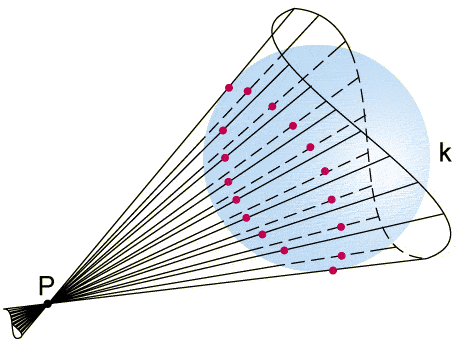
\includegraphics[width=.5\textwidth]{img/tangentialkegel}
 \end{center}
 
 Falls $\Sigma$ eine Großhypersphäre von $\Gamma$ ist, also $\Sigma = \Gamma \cap H$, $H$ Hyperebene durch den Mittelpunkt von $\Gamma$, dann ist $\Phi_\Sigma$ als die Einschränkung der Spiegelung an $H$ definiert.
\end{defn*}

Bezeichne $S(X) := \{ f : X \to X : f$ bijektive Abbildung $\}$.

\begin{defn*}
 Die \emph{verallgemeinerte Möbiusgruppe} $GM(\hat{\real}^n)$ ist definiert als die Untergruppe von $S(\hat{\real}^n)$, die von den Inversionen an Sphären und Spiegelungen an Hyperebenen erzeugt wird. Analog definiert man für die Sphäre $\sphere^n$ die Gruppe $GM(\sphere^n) = S(\sphere^n)$ als die Gruppe, die von Inversionen an Hyperebenen erzeugt wird. 
 \[ \sphere^n = \{ x \in \real^{n+1} : \| x \| = 1 \} \]
 Wir werden sehen, dass $GM(\sphere^n) \simeq GM( \hat{\real}^n )$.
\end{defn*}

\begin{defn*}
  Eine \emph{konforme} Abbildung $f: \real^m \to \real^m$ bewahrt Winkel, also
  \[ \angle(x,y) = \angle(f(x),f(y)). \]

  Eine differenzierbare Abbildung $f: \real^m \to \real^m$ heißt im Punkt $x_0$
  \emph{winkeltreu}, wenn die lineare Approximation $D_{x_0}f$ winkeltreu ist.
  $f$ heißt \emph{winkeltreu} oder \emph{konform}, falls $f$ für alle $x_0 \in
  \real^m$ in $x_0$ winkeltreu ist.

  Die lineare Abbildung $f: \real^m \to \real^m$ ist winkeltreu
  $\Leftrightarrow$ Es existiert $\lambda \ne 0$: $\lambda f$ ist
  orthogonal\footnote{Orthogonale Abbildungen erhalten das Skalarprodukt, sind
    also winkel- und längentreu.}.
\end{defn*}

\clearpage

\begin{thm}
 Sei $\Gamma$ die $n$-Sphäre $\{ x \in \real^{n+1} : \| x-a \| = r \} \subseteq \hat{\real}^{n+1}$. Sei $\Phi_\Gamma: \hat{\real}^{n+1} \to \hat{\real}^{n+1}$ die Inversion an $\Gamma$. Sie hat folgende Eigenschaften:
 \begin{enumerate}[1)]
  \item Sie bildet jede Hyperebene $H$ durch $a$ auf sich selbst ab und operiert auf $H$ als Inversion an $H \cap \Gamma$ ($H \cup \{ \infty \} =: H$)
  \item Sie vertauscht $n$-Sphären $\Sigma$ durch $a$ mit Hyperebenen $H$, die nicht durch $a$ gehen und die Einschränkung auf $\Sigma$ ist die stereographische Projektion von $a$ aus.
  \item Sie bildet die Menge der $n$-Sphären, die nicht durch $a$ gehen, in sich selbst ab.
  \item Sie bildet die Menge der $m$-Sphären und $m$-dimensionalen affinen Unterräume auf sich selbst ab ($0 \le m \le n$).
  \item $\Phi_\Gamma$ ist eine konforme Abbildung.
 \end{enumerate}
\end{thm}

\begin{proof}
  Wir betrachten o.B.d.A. $\Gamma = \Gamma_0$.

  Hyperebenen und Sphären werden durch die Gleichung
  \[ c \| x \|^2 + \angles{b,x} + d = 0 \]
  beschrieben. Die Lösungsmenge ist für
  \begin{itemize}
    \item $c = 0$ eine Hyperebene (falls $b \ne 0$),
    \item $c = 0$, $d \ne 0$ eine Hyperebene durch 0,
    \item $c \ne 0$, $d = 0$ eine Sphäre durch 0.
  \end{itemize}
  Wende die Abbildung $\Phi_{\Gamma_0}(x)$ mit $x \to \frac{x}{\|x\|^2}$ auf die Menge an. Es ergibt sich die Menge, die durch die Gleichung 
  \[ \frac{c}{\| x \|^2} + \frac{\angles{b,x}}{\| x \|^2} + d = 0, \qquad c + \angles{b,x} + d \| x \|^2 = 0 \]
  beschrieben wird. Also haben sich die Rollen von $c$ und $d$ vertauscht.

  Dies beweist die Aussagen 1) bis 3) bis auf die Aussagen über die
  Einschränkungen.

  Zu 1) Die Einschränkung der Spiegelung an $\Gamma$ auf $H \cup \{ \infty \}$
  ist eine Inversion an $H \cap \Gamma$, da es dieselbe Konstruktion ist.
  
  Zu 2) siehe Skizze (rechter Teil). Die Inversion wird am roten Kreis
  ausgeführt, Kreise durch den Mittelpunkt werden auf Hyperebenen abgebildet,
  die nicht den Mittelpunkt berühren.
  
  Die linke Seite illustriert 3), $n$-Sphären, die nicht durch $a$ gehen, werden
  auf andere $n$-Sphären abgebildet, die auch nicht $a$ berühren.
  
  \begin{center}
    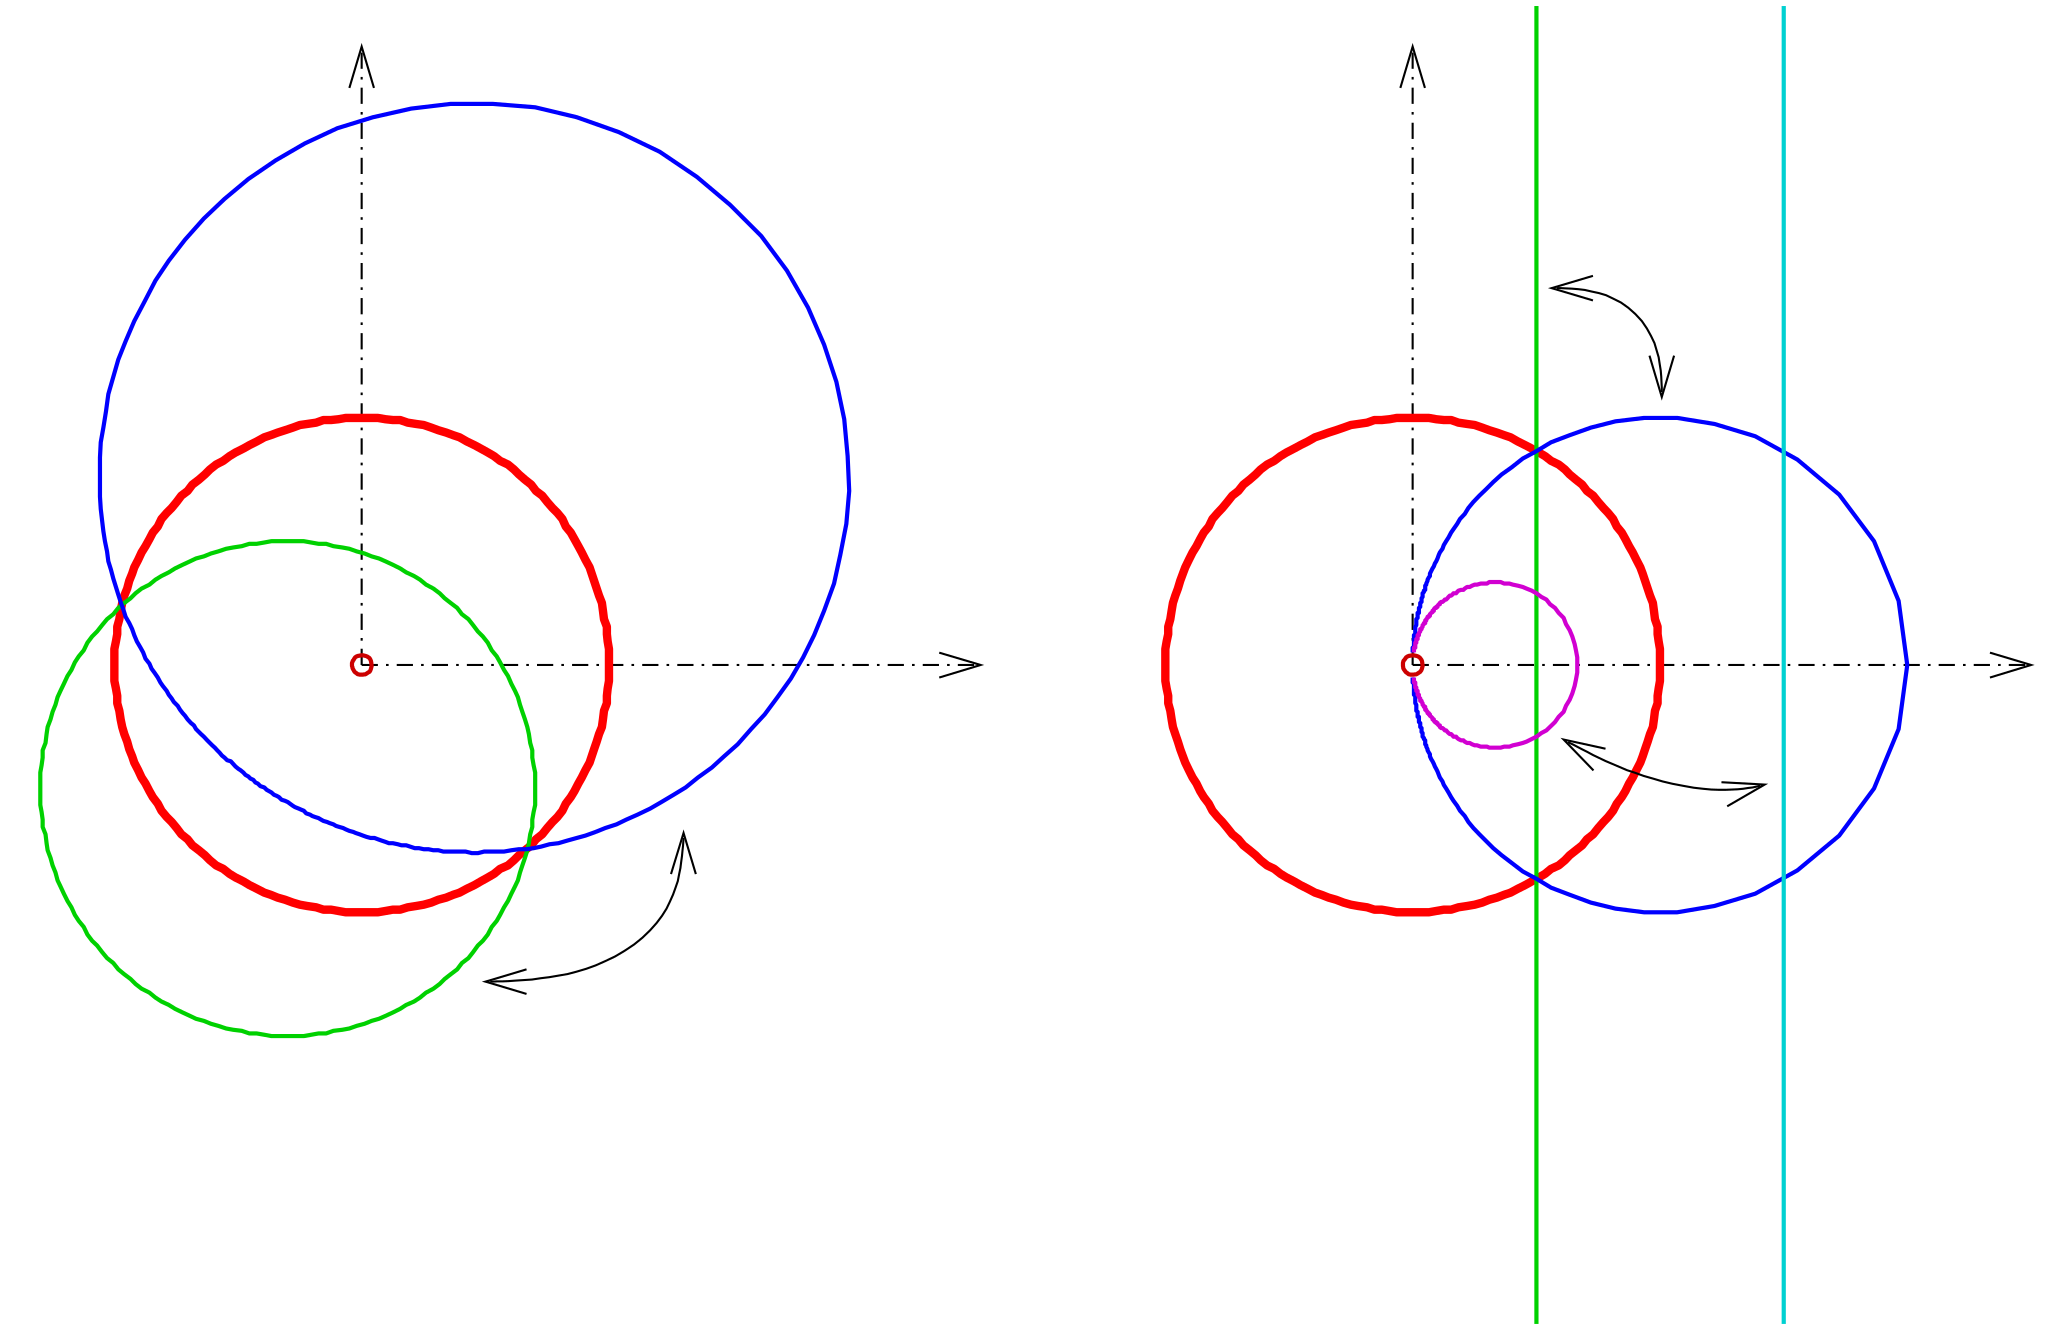
\includegraphics[width=.75\textwidth]{img/Inv-kreis-gerade}
  \end{center}

  Zu 4) Das folgt aus 1) bis 3) durch Bildung von Durchschnitten. $m$-Sphären
  bzw. $m$-dimensionale affine Unterräume (inklusive $\infty$) lassen sich als
  Schnitt von $n$-Sphären beziehungsweise Hyperebenen im $\real^{n+1}$
  darstellen und $\Phi_\Gamma$ ist eine bijektive Abbildung.

  Zu 5) Sei $x \in \real^n$, zunächst $x \notin \Gamma$ und seien zwei
  Tangentialrichtungen $v_1, v_2$ in $x$ gegeben. Betrachte die (eindeutig
  bestimmten) Kreise durch $x$ und $x' = \Phi_\Gamma(x)$, die jeweils in $x$ die
  gegebene Tangentialrichtung haben. (Sonderfall: Gerade, falls $v_i$ in
  Richtung von $\pm(x-x')$ zeigt.)

  $\Phi_\Gamma$ bildet jeden der beiden Kreise auf sich selbst ab, da der
  Bildkreis durch $\Phi_\Gamma(x)$, $x$ und den Schnittkreis durch $\Gamma$ geht
  und ein Kreis durch drei Punkte eindeutig bestimmt ist.

  Zwei Kreise, die sich schneiden, tun das an zwei Punkten und immer im selben
  Winkel. Damit folgt, dass $\Phi_\Gamma$ winkeltreu ist.
\end{proof}

\begin{defn*}
 Seien $x_1, \ldots, x_4 \in \hat{\real}^n$ paarweise verschieden. Dann
 definiere das \emph{Doppelverhältnis} 
 \[ \operatorname{DV}(x_1, x_2, x_3, x_4) := \frac{ \| x_1 - x_2 \| \cdot \| x_3
     - x_4 \| }{ \| x_1 - x_3 \| \cdot \| x_2 - x_4 \| }. \] 
 Achtung: Die Definition ist in der Literatur nicht ganz einheitlich, was die
 Reihenfolge der Punkte betrifft. 

 Falls ein Punkt $\infty$ ist, definiere zum Beispiel
 \[ \operatorname{DV}(x_1, x_2, x_3, \infty) := \frac{\|x_1 - x_2\|}{\|x_1 - x_3\|}. \]
\end{defn*}

Betrachte $x_1, x_2 \in \real^{n+1} \setminus \{ 0 \}$ und o.B.d.A. $f := \Phi_{\Gamma_0},$
\[ f(x) = \frac{x}{\|x\|^2}, \qquad f(0) = \infty, \qquad f(\infty) = 0. \]
Es gilt
\[ \begin{aligned}
    \| f(x_1) - f(x_2) \| 
    &= \left\| \frac{x_1}{\|x_1\|^2} - \frac{x_2}{\|x_2\|^2} \right\| \\
    &= \rez{ \| x_1 \| \cdot \| x_2 \|} 
       \left\| \frac{\| x_2 \|}{\| x_1 \|} x_1 - \frac{\| x_1 \|}{\| x_2 \|} x_2 \right\| \\
    &= \rez{ \| x_1 \| \cdot \| x_2 \|} \sqrt{\| x_2 \|^2 - 2 \angles{x_1,x_2} + \| x_1 \|^2} \\
    &= \frac{ \| x_1 - x_2 \| }{ \| x_1 \| \cdot \| x_2 \| }.
   \end{aligned} \]

Damit erhalten wir
\[ \DV( f(x_1), f(x_2), f(x_3) f(x_4) ) = \frac{ \| x_1 - x_2 \| \cdot \| x_3 -
    x_4 \| }{ \| x_1 - x_3 \| \cdot \| x_2 - x_4 \| } = \DV( x_1, x_2, x_3, x_4
  ). \]
Das Doppelverhältnis ist also invariant unter Inversion an der Einheitssphäre.
Für Inversionen an beliebigen Sphären ist das ``o.B.d.A.'' gerechtfertigt, da
Translationen und Streckungen das Doppelverhältnis offensichtlich bewahren. 

Falls ein $x_i$ gleich 0 oder $\infty$ ist, erfolgt die Rechnung mit der obigen
Definition analog. 

\addtocounter{thm}{-1}
\begin{thm}[Fortsetzung]
 \begin{enumerate}[1)]
  \setcounter{enumi}{5}
  \item Die Inversion an einer Sphäre bewahrt das Doppelverhältnis von vier
    verschiedenen Punkten. 
  \item Die Inversion an $\Gamma$ bildet jede $n$-Sphäre $\Sigma$, die $\Gamma$
    senkrecht schneidet auf sich selbst ab und operiert auf $\Sigma$ als
    Inversion an $\Gamma \cap \Sigma$.
  \item Die Inversion an einer Sphäre $\Gamma$ bzw. an der Hyperebene $\Gamma$
    ist dadurch charakterisiert, dass sie $\Gamma$ punktweise fest lässt und die
    beiden Schnittpunkte von sich schneidenden Kreisen, welche $\Gamma$
    senkrecht schneiden, miteinander vertauscht.
  \item $\Phi_{\Phi_\Gamma(\Sigma)} = \Phi_\Gamma \Phi_\Sigma \Phi_\Gamma$
    (beachte $\Phi_\Gamma^{-1} = \Phi_\Gamma$). 
  \item Die stereographische Projektion $\varphi: \Gamma \to \Pi \cup \{ \infty
    \}$ lässt sich zu einer Inversion $\Phi_\Sigma$ auf $\real^{n+1}$ fortsetzen
    (wobei $\Gamma \subseteq \hat{\real}^{n+1}$ Hypersphäre, $\Pi \subseteq
    \real^{n+1}$ Hyperebene). Folglich hat die stereographische Projektion
    ebenfalls die Eigenschaften 4) - 6). 
  \item Seien $\Gamma, \Gamma' \subseteq \hat{\real}^n$ zwei $k$-Sphären oder
    $k$-Ebenen ($k$-dimensionale affine Unterräume inklusive $\infty$). Dann ist
    in natürlicher Weise $GM(\Gamma) \subseteq GM(\hat{\real}^n)$. Ferner sind
    $GM(\Gamma)$ und $GM(\Gamma')$ in $GM(\hat{\real}^n)$ konjugierte
    Untergruppen, also insbesondere $GM(\Gamma) \simeq GM(\Gamma')$ und $GM(S^n)
    \simeq GM(\hat{\real}^n)$. 
  \item Alle Abbildungen in $GM(\hat{\real}^n)$ (verallgemeinerte
    Möbiustransformationen) erfüllen 4) - 6). 
 \end{enumerate}
\end{thm}

\begin{proof}
 \begin{enumerate}[1)]
  \setcounter{enumi}{5}
  \item Wurde bereits gezeigt.
  \item Das folgt direkt aus 3) und 5).
  \item Klar mit 3) und 5).
  \item Das folgt aus 8): Sei $x \in \hat{\real}^n$ beliebig.
  
  Betrachte zwei Kreise, die sich in $x$ schneiden und $\Phi_\Gamma(\Sigma)$ senkrecht schneiden. Sie schneiden sich also das zweite Mal in $\Phi_{\Phi_\Gamma(\Sigma)}$. 
  
  Die Bilder dieser Kreise unter $\Phi_\Gamma$ schneiden $\Phi_\Gamma(\Phi_\Gamma(\Sigma)) = \Sigma$ senkrecht und schneiden sich in $\Phi_\Sigma(x)$ und folglich das zweite Mal in $\Phi_\Sigma \Phi_\Gamma(x)$. Daraus folgt, dass für alle $x$ $\Phi_\Sigma \Phi_\Gamma(x)$ mit $\Phi_\Gamma \Phi_{\Phi_\Gamma(\Sigma)}(x)$ übereinstimmt und damit ist
  \[ \Phi_{\Phi_\Gamma(\Sigma)}= \Phi_\Gamma^{-1} \Phi_\Sigma \Phi_\Gamma = \Phi_\Gamma \Phi_\Sigma \Phi_\Gamma. \]
  \item Betrachte eine Sphäre $\Sigma$ mit Mittelpunkt $a \in \Gamma$. Die
    Inversion an dieser Sphäre operiert auf $\Gamma$ als stereographische
    Projektion.
  \item $GM(\hat{\real}^n)$ enthält alle Spiegelungen an Hyperebenen, also alle
    Bewegungen. Ferner ent\-hält sie alle Streckungen (betrachte einfach die
    Konjugation von zwei Inversionen an konzentrischen Sphären). Mit einer
    Inversion können wir einen $k$-dimensionalen affinen Unterraum auf eine
    $k$-dimensionale Sphäre abbilden und umgekehrt.
  
    Damit folgt 11) aus 9).
  \item Das ist klar, da die Eigenschaften in 4) bis 6) unter Komposition
    erhalten bleiben. \qedhere
 \end{enumerate}
\end{proof}

\textbf{Anwendungsbeispiel.} Gegeben sei eine Kreisschar durch zwei Punkte. Gibt
es eine weitere Kreisschar, die alle Kreise der ersten Schar senkrecht
schneidet? Wende die Inversion an einem Kreis an, der einen der beiden Punkte als
Mittelpunkt hat.

Inversionen an Sphären und Spiegelungen an Hyperebenen sind
orientierungsumkehrend. Eine Untergruppe vom $GM(\hat{\real}^n)$ sind daher auch
die orientierungserhaltenden Abbildungen in $GM(\hat{\real}^n)$.

Dies ist die Gruppe aller Kompositionen einer geraden Anzahl von Inversionen
(oder Spiegelungen an Hyperebenen). Diese Untergruppe $M(\hat{\real}^n)$ heißt
die Gruppe der Möbius\-trans\-formationen (meistens $M(\hat{\complex})$).

$M(\hat{\real}^n)$ enthält alle Translationen, Streckungen, Drehungen
(Inversionen an zwei konzentrischen Kreisen). In $\complex$:
\begin{itemize}
  \item $z \mapsto z + t$ ... Translation
  \item $z \mapsto a \cdot z$ ... Drehstreckung für $a \in \complex \setminus \{
    0 \}$
  \item $z \mapsto \rez{z}$ ... Komposition der Inversion am Einheitskreis in
    $\hat{\complex}$ mit der Spiegelung an der reellen Achse. ($\rez{z} = \frac{\obar{z}}{|z|^2}$)
\end{itemize}

Die Abbildungen dieser Art erzeugen die Möbiusgruppe $M(\hat{\complex})$ mit
\[ M(\hat{\complex}) = \left\{ f: \hat{\complex} \to \hat{\complex} : f(z) = \frac{ az +
    b}{c z + d} \text{ mit } ad - bc = 1 \right\}. \]
Weitere Diskussion in der Übung.

\subsection{Sphärische und elliptische Geometrie}
Wir betrachten die Geometrie auf $\sphere^n \subseteq \real^{n+1}$
(Einheitssphäre). Die Metrik auf $\sphere^n$ wird definiert durch
\[ d(x,y) = \arccos \angles{x,y} \qquad \in [0,\pi] \]
für $x,y \in \sphere^n$ (also $\| x \| = \| y \| = 1$).

Es gilt:
\begin{enumerate}
  \item $d$ ist eine Metrik auf $\sphere^n$.
  \item $d(x,y) + d(y,z) = d(x,y)$ $\Leftrightarrow$ $x,y,z$ liegen auf einem
    Großkreis (also sind $x,y,z$ linear abhängig) und $d(x,y) + d(y,z) \le
    \pi$ ($y$ liegt auf dem kürzeren Bogen, der $x$ und $z$ verbindet).
  \item Der kleinere der beiden Großkreisbögen, die $x$ und $y$ verbinden, hat
    Länge $d(x,y)$ und ist der kürzeste Abstand.
  \item Die Großkreise sind also die lokal kürzesten Verbindungen (in der
    Differentialgeometrie: geodätisch).
\end{enumerate}

\subsection{Geodätische Dreiecke auf der \texorpdfstring{$\sphere^2$}{S2}}

Seien $x,y,z$ drei Punkte auf $\sphere^2$, so dass $x,y,z,-x,-y,-z$ paarweise
verschieden sind.

Verbinde $x$ mit $y$, $y$ mit $z$ und $z$ mit $x$ durch die kürzesten
Verbindungen. Dadurch werden Zweiecke aufgespannt, die $x$ und $-x$, $y$ und
$-y$ sowie $z$ und $-z$ verbinden, ihre Öffnungswinkel seien $A$, $B$ und $C$.

Die Oberfläche der $\sphere^2$ ist $4 \pi$, der Flächeninhalt eines Zweiecks mit
Öffnungswinkel $A$ ist gleich $2A$.

Also folgt für die Fläche des Dreiecks $\Delta$:
\begin{align*}
    \Delta + \Delta_A &= 2A \tag{1} \\
    \Delta + \Delta_B &= 2B \tag{2} \\
    \Delta + \Delta_C &= 2C \tag{3} \\
    2(\Delta + \Delta_A + \Delta_B + \Delta_C) &= 4 \pi. \tag{4}
\end{align*}

Mit $(1) + (2) + (3) - \rez{2} (4)$ erhält man
\[ 2 \Delta = 2 (A+B+C) - 2 \pi, \]
also
\[ \Delta = A + B + C - \pi. \]

Wir haben damit gezeigt:

\newpage

\begin{thm}
  Der Flächeninhalt eines geodätischen Dreiecks auf der $\sphere^2$ ist
  \[ \Delta = A + B + C - \pi, \]
  wobei $A,B,C$ die drei Winkel des Dreiecks sind.
\end{thm}

Sei $x,y,z$ ein geodätisches Dreieck mit Seitenlänge $< \pi$. Die Winkel des
Dreiecks seien $A,B,C$, die Seiten $a,b,c$.

Ein \emph{Tangentialvektor} in $x$ ist gegeben durch
\[ u_1 = \frac{y-\angles{y,x}x}{\|y-\angles{y,x}x\|}, \]
denn $u_1 \perp x$, $\| u_1 \| = 1$, $\angles{u_1,y} = 0$. Analog folgt
\[ u_2 = \frac{z-\angles{z,x}x}{\|z-\angles{z,x}x\|}. \]

Nun können wir den Öffnungswinkel $A = \arccos \angles{u_1, u_2}$ bestimmen:
\[ \cos A = \angles{u_1,u_2} =
  \frac{\angles{y,z} - \angles{y,x} \angles{x,z}
    - \angles{z,x} \angles{x,y} + \angles{y,x} \angles{z,x}}
  {\sqrt{1 - 2 \angles{y,x}^2 + \angles{y,x}^2} \cdot
    \sqrt{1 - 2 \angles{z,x}^2 + \angles{z,x}^2} }. \]
Wegen $\sqrt{1 - \angles{y,x}^2} = \sqrt{1 - \cos^2 c} = \sin c$ und analog für
$\sin b$, $\cos c$ und $\cos b$ gilt also der sogenannte \emph{Kosinussatz}:
\[ \cos A = \frac{ \cos a - \cos b \cdot \cos c }{ \sin b \cdot \sin c }. \]

Es gilt
\[ \begin{aligned}
    \sin A &= \sqrt{1-\cos^2 A} \\
    &= \frac{\sqrt{\sin^2 b \sin^2 c - (\cos a - \cos b \cos c)^2}}{\sin b \cdot
      \sin c} \\
    &= \frac{\sqrt{(1-\cos^2 b)(1-\cos^2 c) - \cos^2 a + 2 \cos a \cos b \cos c
        - \cos^2 b \cos^2 c}}{\sin b \cdot \sin c} \\
    &= \frac{\sqrt{1 - \cos^2 a - \cos^2 b - \cos^2 c + 2 \cos a \cos b \cos
        c}}{\sin b \cdot \sin c}.
  \end{aligned} \]
Man kann die Berechnung analog für $B$ und $C$ durchführen und erhält
\[ \frac{\sin A}{\sin a} = \frac{\sin B}{\sin b} = \frac{\sin C}{\sin c}. \]

\subsection{Elliptische Geometrie}
Betrachte
\[ \begin{aligned}
    \proj(\real^{n+1}) &= \{ [x] : x \in \real^{n+1} \setminus \{0\}\} \\
    &= \{ [x] : x \in \sphere^1 \} = \sphere^n_\pm.
  \end{aligned} \]
Die natürliche Metrik auf $\real^{p^n}$ ($\proj(\real^{n+1})$ mit Längen und
Winkeln) ist
\[ d( [x], [y] ) = \arccos | \angles{x,y} | \le \frac{\pi}{2} \]
für $x, y \in \sphere^n$.

Die Geraden sind die Großkreise mit gegenüberliegenden Punkten identifiziert,
haben also Länge $\pi$.

In $\real^{p^2}$ gibt es ``nicht nullhomotope Dreiecke''.

\subsection{Modelle des hyperbolischen Raumes}
Der hyperbolische Raum wird mit $\real H^n$ bezeichnet.

\textbf{1. Modell.} (Klein'sches Modell, e-Modell)
\begin{itemize}
  \item Menge der \emph{Punkte}: Offene Einheitskugel
  \item \emph{Geraden} sind nichtleere Schnitte von Geraden in $\real^n$ mit $B^n$.
  \item Zwei Geraden (in diesem Modell) heißen \emph{parallel}, wenn sie sich
    auf dem Rand von $B^n$ schneiden.
\end{itemize}

\textbf{Inzidenzgeometrische Eigenschaften.}
\begin{itemize}
  \item Durch je zwei Punkte geht genau eine Gerade.
  \item Je zwei Geraden schneiden sich in höchstens einem Punkt.
  \item Zu jeder Geraden und jedem Punkt, der nicht auf der Geraden liegt, gibt
    es genau zwei Parallelen.
\end{itemize}


\textbf{Achtung!} Parallelität ist im $\real H^n$ \emph{keine
  Äquivalenzrelation}. Sinnvoller wäre es also, statt Geraden Strahlen zu
betrachten und parallele Strahlen.

\textbf{2. Modell} (Projektives Modell, p-Modell)
\begin{itemize}
  \item Fasse $B^n$ als Teilmenge von $\proj(\real^{n+1})$ auf.
  \[ x (\in \real^n) \quad \mapsto \quad \left[ \pmat{1 \\ x} \right] (\in
    \proj(\real^{n+1})). \]
  \item Menge der Punkte: $\real H^n := \left\{ \left[ \pmat{1 \\ x} \right]
      : x \in \real^n, \| x \| < 1 \right\}$.
  \item \emph{Geraden} sind nichtleere Schnitte von Geraden im
    $\proj(\real^{n+1})$ mit $\real H^n$.
  \item \emph{$k$-dimensionale Unterräume} sind nichtleere Schnitte von
    $k$-dimensionalen projektiven Unterräumen mit $\real H^n$.
\end{itemize}

Wir betrachten nun den $\real^{n+1}$ mit einer anderen Bilinearform, nämlich
\[ \angles{x,y}_- := x_1 y_1 - \sum_{j=2}^{n+1} x_j y_j, \]
wobei $x = (x_1, \ldots, x_{n+1})$ und $y = (y_1, \ldots, y_{n+1})$. Definiere
\[ J := \pmat{
    1 & 0 & \cdots & 0 \\
    0 & -1 \\
    \vdots & & \ddots \\
    0 & & & -1
  }. \]
Das ist die zu $\angles{\cdot,\cdot}_-$ gehörige Matrix.
\[ \angles{x,y}_- = x^T J y, \qquad \| x \|_- := \sqrt{|\angles{x,x}_-|}. \]

Nun können wir den $\real H^n$ so betrachten:
\[ \begin{aligned}
    \real H^n &= \{ [x] : x \in \real^{n+1}, \angles{x,x}_- > 0 \} \\
  &= \left\{ \left[ \pmat{ 1 \\ x_2 \\ \cdots \\ x_{n+1} } \right] : x_2^2 +
    \ldots + x_{n+1}^2 < 1  \right\} \\
  &= \{ [x] : x \in \real^{n+1}, \angles{x,x}_- = 1, x_1 > 0 \}.
\end{aligned} \]
Die Gleichung
\[ x_1^2 - x_2^2 - \ldots - x_{n+1}^2 = 1 \]
beschreibt ein zweischaliges Rotationshyperboloid.

\textbf{Zur Erinnerung.} Aus der Analysis ist bekannt
\begin{align*}
  \cos a &= \rez{2} (e^{ia} + e^{-ia}) & \cosh a &= \rez{2} (e^a + e^{-a}) \\
  \sin a &= \rez{2i} (e^{ia} - e^{-ia}) & \sinh a &= \rez{2} (e^a - e^{-a}),
\end{align*}
sowie
\[ \cosh^2 a - \sinh^2 a = 1. \]

Die Umkehrfunktionen sind
\begin{align*}
  \operatorname{arcosh} a &= \ln( a + \sqrt{a^2 - 1}), \\
  \operatorname{arsinh} a &= \ln( a + \sqrt{a^2 + 1}).
\end{align*}

\begin{defn*}
  Der hyperbolische Abstand von $[x]$, $[y] \in \real H^n$ ist
  \[ d([x],[y]) := \operatorname{arcosh} \frac{|\angles{x,y}_-|}{\|x\|_- \|y\|_-}.\]
  Wir müssen nachweisen, dass dadurch eine Metrik definiert ist. Dass $d(\cdot, \cdot)$ wohldefiniert, symmetrisch und $\ge 0$ ist, ist klar.

  Seien $x =\pmat{x_1 \\ \tilde{x}}$, $y =\pmat{y_1 \\ \tilde{y}}$ mit $x_1, y_1
  > 0$. O.B.d.A. sei $\angles{x,x}_- = \angles{y,y}_- = 1$. Dann gilt
  \[ x_1^2 - \| \tilde{x} \|^2 = y_1^2 - \| \tilde{y} \|^2 = 1. \]
  Damit folgt
  \[ \angles{x,y}_- = x_1 y_1 - \angles{\tilde{x},\tilde{y}} =\sqrt{1 + \|
      \tilde{x} \|^2} \cdot \sqrt{1 + \| \tilde{y} \|^2} -
    \angles{\tilde{x},\tilde{y}} \ge 0,\]
  denn
  \[ (1+\|\tilde{x}\|^2) (1+\|\tilde{y}\|^2) \ge ( 1 +
    \angles{\tilde{x},\tilde{y}})^2, \]
  wobei Gleichheit genau dann gilt, wenn $\tilde{x} = \tilde{y}$. Damit gilt
  $d(x,y) = 0$ genau dann, wenn $x = y$.
\end{defn*}

\subsection{Die Isometriegruppe von \texorpdfstring{$\real H^n$}{RH2}}
\begin{defn*}
  \begin{align*}
    O(1,n) 
    &= \{ A \in \real^{n+1,n+1} : A^T J A = J \} \\
    &= \{ A \in \real^{n+1,n+1} : \text{ Für alle $x,y \in \real^{n+1}$ gilt } 
      \angles{x,y}_- = \angles{Ax,Ay}_- \},
  \end{align*}
  denn
  \[x^T J y = \angles{x,y}_- = \angles{Ax,Ay}_- = x^T A^T J A y\]
  für alle $x,y \in \real^{n+1}$, also $A^T J  A = J$.

  Damit ist $A \in O(1,n)$, falls für die Spaltenvektoren $a_1, \ldots, a_{n+1}$
  gilt:
  \begin{align*}
    \angles{a_1, a_1}_- &= 1, \\
    \angles{a_i, a_i} &= -1 & \text{für alle } i = 2, \ldots, n+1, \\
    \angles{a_i, a_j} &= 0 & \text{für } i \ne j.
  \end{align*}
\end{defn*}

Für die Repräsentanten der Punkte in $\real H^n$ können wir voraussetzen $x_1
\ge 1.$

In $O(1,n)$ sind die linearen Abbildungen, die das zweischalige Hyperboloid $\{
x : \angles{x,y}_- = 1 \}$ auf sich abbilden.

Eine Untergruppe davon sind diejenigen, die jede der beiden Komponenten auf sich
abbilden, das heißt diejenigen Matrizen mit $a_{11} > 0$ (also sogar $a_{11} \ge
1$ wegen $\angles{a_1,a_1}_- = 1$).

\begin{defn*}
  \[ O_+(1,n) := \{ A \in O(1,n) : a_{11} > 0 \}. \]
  Die Abbildungen in $O_+(1,n)$ sind Isometrien des $\real H^n$, genauer ist für
  $A \in O_+(1,n)$ die Abbldung $[x] \mapsto [Ax]$ eine Isometrie.

  Die Abbildung $O_+(1,n) \to \operatorname{Iso}( \real H^n )$ ist injektiv.
\end{defn*}

\begin{defn*}
  Eine \emph{hyperbolische Spiegelung} (h-Spiegelung) ist eine Isometrie $f:
  \real H^n \to \real H^n$, die eine Hyperebene (punktweise) fest lässt, mit $f
  \ne \id$.
\end{defn*}

\begin{exmp*}
  Sei
  \[ A = \begin{pmatrix}
      \cosh s & - \sinh s & 0 & \cdots & 0 \\
      \sinh s & - \cosh s & 0 & \cdots & 0 \\
      0 & 0 & 1 \\
      \vdots & \vdots & & \ddots \\
      0 & 0 & & & 1
    \end{pmatrix}
  \]
  Wegen $\cosh^2 s - \sinh^2 s = 1$ ist $A \in O_+(1,n)$.

  Betrachte $\pmat{\cosh s & - \sinh s \\ \sinh s & - \cosh s}$. Wir ermitteln
  die Eigenwerte:
  \[ (\cosh s - \lambda)(- \cosh s - \lambda) + \sinh^2 s =
    - \cosh^2 s + \lambda^2 + \sinh^2 s = \lambda^2 -1 = 0. \]
  Also folgt $\lambda_{1,2} = \pm 1$.

  Bestimme nun einen Eigenvektor der Form $\pmat{ 1 \\ y }$ zu $\lambda_2 = -1$.
  Aus der ersten Zeile von
  \[ \pmat{\cosh s & - \sinh s \\ \sinh s & - \cosh s} \pmat{ 1 \\ y } = \pmat{
      1 \\ y } \]
  folgt $1 = - \cosh s + y \sinh s$ und damit
  \begin{align*}
    y &= \frac{1 + \cosh s}{\sinh s} = \frac{2 + e^s + e^{-s}}{e^s - e^{-s}} \\
      &= \frac{(e^{s/2} + e^{-s/2})^2}{(e^{s/2}+e^{-s/2})(e^{s/2}-e^{-s/2})}
        = \frac{e^{s/2}+e^{-s/2}}{e^{s/2}-e^{-s/2}} \\
    &= \coth \frac{s}{2}.
  \end{align*}
  Für $\lambda_1 = 1$ gilt $1 = \cosh s - y \sinh s$ und damit
  \[ y = \frac{-1 + \cosh s}{\sinh s} = \tanh \frac{s}{2}. \]

Also definiert $A$ im p-Modell eine h-Spiegelung und ist die Einschränkung einer
Zentralkollineation, deren Achse die Hyperebene
\[ \left\{ \left[ \pmat{ 1 \\ \tanh \frac{s}{2} \\ a } \right] : a \in
    \real^{n-1} \right\} \]
in $\proj( \real^{n+1})$ ist. Das Zentrum ist die Spitze des Tangentialkegels an
die Einheitskugel (in $\real H^n$) an den Schnitt der Hyperebene mit
$\obar{\real H}^n$,
\[ \left[  \pmat{1 \\ 0 \\ \vdots \\ 0} \right] \mapsto  \left[ \pmat{ \cosh s
      \\ \sinh s \\ \vdots \\ 0} \right] = \left[\pmat{ 1 \\ \tanh s \\ \vdots \\
      0}\right]. \]
\end{exmp*}

\begin{rmrk*}
Für $C \in O_+(1,n)$ gilt
\[ C \pmat{1 \\ 0 \\ \vdots \\ 0} = \pmat{1 \\ 0 \\ \vdots \\ 0} \qRq \exists B
  \in O(n) : C =
  \begin{pmatrix}
    1 & 0 & \cdots & 0 \\
    0 \\
    \vdots & & B \\
    0 
  \end{pmatrix}. \]
Wir betrachten die Matrizen in $O_+(1,n)$ als Isometrien des $\real H^n$,
nämlich $A([x]) := [Ax]$.
\end{rmrk*}

\begin{thm}
  \begin{enumerate}[a)]
  \item $O_+(1,n)$ operiert transitiv auf der Menge der Punktepaare von $\real
    H^n$ mit festem Abstand $a$.
  \item Jedes Element aus $O_+(1,n)$, lässt sich als Produkt von höchstens $n+1$
    h-Spiegelungen schreiben.
  \end{enumerate}
\end{thm}

\begin{proof}
  Zu a): Zunächst zeigen wir, dass jeder Punkt in $\real H^n$ durch eine
  h-Spiegelung auf $O := [ \pmat{1 & 0 & \cdots & 0}^T ]$ abgebildet werden
  kann.
  \[ A = \begin{pmatrix}
      \cosh s & - \sinh s & 0 & \cdots & 0 \\
      \sinh s & - \cosh s \\
      0 & 0 \\
      \vdots & \vdots & & E_{n-1} \\
      0 & 0
    \end{pmatrix}
    \qRq
  AO = \left[ \pmat{ \cosh s \\ \sinh s \\ \vdots \\ 0} \right] = \left[\pmat{ 1
      \\ \tanh s \\ \vdots \\ 0} \right]. \]
  Der Wertebereich von $\tanh s$ ist $(-1,1)$, also ist jeder Punkt der h-Geraden
  \[ \left[ \real \pmat{ 1 \\ 0 \\ 0 \\ \vdots \\ 0} + \real \pmat{ 1 \\ 1 \\ 0
        \\ \vdots \\ 0} \right] \cap \real H^n \]
  das Bild von $O$ unter einer h-Spiegelung der obigen Form.

  Sei $\left[ \pmat{1 \\ x} \right] \in \real H^n$ beliebig und $s =
  \operatorname{artanh} (\|x\|)$. Die h-Spiegelung an der Hyperebene orthogonal
  (im e-Modell) zu $x$ und durch $\frac{x}{\|x\|} \tanh \frac{s}{2}$ vertauscht
  $O$ und $\left[ \pmat{1 \\ x} \right]$.

  Seien nun $[x_1], [x_2], [y_1], [y_2] \in \real H^n$ mit $d([x_1],[x_2]) =
  d([y_1],[y_2])$. Dann gibt es $\varphi_1, \varphi_2 \in O_+(1,n)$ mit
  \[ \varphi_1(x_1) = \pmat{1 \\ 0 \\ \cdots \\ 0}, \qquad \varphi_2(y_1) =
    \pmat{1 \\ 0 \\ \cdots \\ 0}. \]
  Wegen
  \[ d(O, [\varphi_1(x_2)]) = d([\varphi_1(x_1)], [\varphi_1(x_2)]) =
    d([y_1],[y_2]) = d(O,[\varphi_2(y_2)]) \]
  gibt es $\varphi_3= \pmat{1 & 0 \\ 0 & B}$ mit $B \in O(n)$ mit $[\varphi_3
  \varphi_1(x_2)] = [\varphi_2(x_2)]$. Also bildet $\varphi_3^{-1} \circ
  \varphi_3 \circ \varphi_1$ $x_1$ auf $y_1$ und $x_2$ auf $y_2$ ab.

  Zu b): Sei $A \in O_+(1,n)$ beliebig und $x = A \cdot (1,0,\ldots,0)^T$. Dann
  gibt es eine h-Spiegelung $S_0$ mit $S_0 x = (1,0,\ldots,0)^T$. Damit gilt
  \[ S_0 A \cdot \pmat{1 \\ 0 \\ \vdots \\ 0} = \pmat{1 \\ 0 \\ \vdots \\ 0} \]
  und folglich ist $S_0 A$ von der Form $\pmat{1 & 0 \\ 0 & B}$ mit $B \in
  O(n)$. $B$ ist ein Produkt von höchstens $n$ Spiegelungen an Hyperebenen des
  $\real^n$.

  Eine Spiegelung im e-Modell an einer Hyperebene durch $O$ des $\real^n$ ist
  auch eine h-Spiegelung ($C \in O(n) \mapsto \pmat{1 & 0 \\ 0 & C}$). Also ist
  $A$ Produkt von höchstens $n+1$ h-Spiegelungen.
\end{proof}

\subsection{Das konforme Modell des hyperbolischen Raumes}
Stereographische Projektion
\[ \varphi: \sphere^n \to \hat{\real}^n, \qquad \varphi(x,t) = \frac{x}{1-t}, \]
wobei $t^2 + \|x\|^2 = 1$, $t \ne 1$. $\varphi(0,1) = \infty$.

\textbf{Übergang vom e-Modell zum k-Modell.} Dieser erfolgt durch eine geometrische
Konstruktion. Bilde zunächst $B^n$ auf die untere Halbsphäre der $\sphere^n
\subseteq \real^{n+1}$ durch orthogonale Projektion ab.

Bilde die untere Halbsphäre anschließend durch stereographische Projektion vom
Nordpol aus auf die offene Kugel $B^n$ ab.

Eine h-Gerade im e-Modell (Schnitt von Gerade mit $B^n$) wird durch die
orthogonale Projektion auf einen Kreisbogen abgebildet (auf der unteren
Halbsphäre), der den Rand von $B^n$ senkrecht schneidet. Durch die
stereographische Projektion (winkeltreu!) wird dieser Kreis auf einen Kreis oder
eine Gerade in $B^n$ abgebildet, der den Rand senkrecht schneidet.

Der Rand von $B^n$ bleibt unter beiden Abbildungen punktweise fest. Damit
erhalten wir das \emph{konforme Modell}.

\textbf{k-Modell.}
\begin{itemize}
  \item Menge der \emph{Punkte}: $B^n = \{ x \in \real^n : \| x \| \le 1 \}$
  \item \emph{Geraden} sind Schnitte von Kreisen, die $\partial B^n$ senkrecht
    schneiden mit $B^n$ bzw. Schnitte von Geraden durch 0 mit $B^n$.
  \item \emph{$m$-dimensionale Unterräume} sind Schnitte von $m$-Sphären, die
    $\partial B^n$ senkrecht schneiden, mit $B^n$.
\end{itemize}

\textbf{Direkter Übergang zwischen den Modellen.} Sei $x \in B^n$. Projektion
senkrecht nach unten auf $\sphere^n \subseteq \real^{n+1}$ ergibt
\[ \pmat{ x \\ - \sqrt{1-\|x\|^2}} \mapsto \frac{x}{1 + \sqrt{1-\|x\|^2}}, \]
wobei $\mapsto$ die stereographische Projektion ist.

Die Abbildung $F: B^n \to B^n$ ist definiert durch
\[ F(x) := \frac{x}{1+\sqrt{1-\|x\|^2}}. \]
Sie bildet $x$ im e-Modell auf den entsprechenden Punkt im k-Modell ab.

\begin{center}
\begin{tabular}{c|c|c}
  e-Modell & p-Modell & k-Modell \\
  \hline
  $x$ & $\left[ \pmat{1\\x} \right]$ & $\cfrac{x}{1+\sqrt{1-\|x\|^2}}$ \\[5pt]
  $\cfrac{x}{a}$ & $\left[ \pmat{a\\x} \right]$ & $\cfrac{x}{a+\sqrt{a^2-\|x\|^2}}$
\end{tabular}
\end{center}
mit $\|x\|^2 < a^2$.

Sei $H$ eine Hyperebene, die $B^n$ schneidet, bezeichne $\Psi_H$ die
$h$-Spiegelung an $H$ (im $e$-Modell), also ist $\Psi_H$ die Einschränkung der Zentralkollineation, welche $B^n$ auf sich abbildet mit Achse $H$ und deren Zentrum die Spitze des Tangentialkegels an $B^n$ in $\partial B^n \cap H$ ist.

\begin{thm}[Hyperbolische Spiegelungen im k-Modell]
 Sei $\Phi_{F(H)}$ die Inversion (Spiegelung) an der Sphäre $F(H)$. Dann gilt auf $B^n$:
 \[ F \circ \Psi_H = \Phi_{F(H)} \circ F, \]
 das heißt die h-Spiegelung an der h-Hyperebene $H \cap B^n$ im e-Modell entspricht genau der Inversion (Spiegelung) an der Sphäre $F(H)$ im k-Modell.
\end{thm}

\begin{proof}
 Auf dem Rand $\partial B^n$ stimmen $\Psi_H$ und $\Phi_{F(H)}$ überein.
 
 1. Fall: Für $x \in H$ ist $F(x) \in F(H)$, also $F \circ \Psi_H(x) = F(x) = O_{F(H)} F(x)$.
 
 2. Fall: Sei $x \in B^n \setminus H$. Sei $E$ die Ebene durch $0$, $x$ und $z$ (Zentrum von $\Psi_H$). $E$ schneidet $\partial B^n = \sphere^{n-1}$ in einem Großkreis. Wir können die Konstruktion in $E$ durchführen (Die Einschränkung von $E$ auf $\partial B^n$ wird unter den betrachteten Abbildungen auf sich abgebildet). 
 
 Die Konstruktion der Bildpunkte zeigt, dass $F \circ \Psi_H(x) = \Phi_{F(H)} F(x)$ gilt. Wir verwenden dabei, dass die Abbildungen $\Phi_{F(H)}$ und $\Psi_H$ auf $\partial B^n$ übereinstimmen und wegen der Winkeltreue von $\Phi_{F(H)}$ Kreise, die $\partial B^n$ senkrecht schneiden, wieder auf Kreise überführt werden, die $\partial B^n$ senkrecht schneiden.
\end{proof}

\begin{rmrk*}
 \begin{enumerate}[1)]
  \item Die Abbildungen $\Psi_H$ und $\Phi_{F(H)}$ auf $\sphere^{n-1} = \partial B^n$ sind die Inversion der $\sphere^{n-1}$ an $H \cap \sphere^{n-1}$.
  \item Jede Spiegelung der $\sphere^{n-1}$ an einer $(n-2)$-Sphäre $\Sigma \subseteq \sphere^{n-1}$ lässt sich einerseits \emph{ein\-deu\-tig} zu einer Spiegelung an der $(n-1)$-Sphäre, die die $\sphere^{n-1}$ in $\Sigma$ schneidet, fortsetzen, andererseits zu einer Zentralkollineation $\Psi_H$ mit $\Sigma = H \cap \sphere^n$.
 \end{enumerate}
\end{rmrk*}

\begin{thm}
 Die h-Winkel stimmen mit den Winkeln im k-Modell überein.
\end{thm}

\begin{proof}
 Zwei h-Strahlen $g_1$, $g_2$ von einem Punkt $x \in B^n$ lassen sich durch eine h-Spiegelung auf Strahlen abbilden, die von 0 (im e-Modell bzw. im k-Modell) ausgehen. Der Winkel $\alpha$ zwischen diesen Strahlen stimmt im e-Modell und im k-Modell überein und $\alpha$ ist auch der h-Winkel.
 
 Wir wissen, dass eine h-Spiegelung nach Satz 4.3 einer Inversion an einer Sphäre im k-Modell entspricht. Diese Inversionen sind winkeltreu, also stimmen auch die Winkel zwischen den h-Strahlen im k-Modell mit den Winkeln zwischen $g_1$ und $g_2$ überein.
\end{proof}

\begin{thm}
 Es gilt 
 \[ GM(\hat{\real}^n) \simeq GM( \sphere^n ) \simeq O_+ (1, n+1). \]
 Ferner gilt: Jede Möbiustransformation $f \in GM(\sphere^n)$ bzw. $f \in GM(\hat{\real}^n)$ lässt sich als Produkt von höchstens $n+2$ Spiegelungen an $(n-1)$-Sphären schreiben.
\end{thm}

\begin{proof}
 Wir haben schon gezeigt, dass $GM(\hat{\real}^n) \simeq GM( \sphere^n )$. Sei $f \in GM(\sphere^n)$, das heißt $f$ lässt sich als Produkt (Komposition) von Spiegelungen an $(n-1)$-Sphären darstellen.
 
 Diese lassen sich jeweils \emph{eindeutig} zu Zentralkollineationen fortsetzen, welche $B^{n+1}$ auf sich selbst abbilden (also h-Spiegelungen im e-Modell). Diese lassen sich jedoch durch eine Matrix $A \in O_+(1,n+1)$ darstellen. Damit ist $f$ die Einschränkung einer Kollineation $\obar{f}: \proj(\real^{n+2}) \to \proj(\real^{n+2})$ auf $O_+(1,n+1)$. 
 
 Diese Kollineation $\obar{f}$ ist durch $f$ eindeutig bestimmt: Sei $x \in \proj(\real^{n+2})$. Dann gibt es $a_1, a_2, b_1, b_2 \in \sphere^n (\subseteq \proj( \real^{n+2} ) )$ mit $x = a_1 a_2 \cap b_1 b_2$, also $f(\obar{x}) = f(a_1) f(a_2) \cap f(b_1) f(b_2)$.
 
 Damit erhalten wir eine Abbildung $\tilde{f}: GM(\sphere^n) \to O_+(1,n+1)$. Sie ist offenbar mit Komposition verträglich, also ein Gruppenhomomorphismus. 
 
 Ferner ist $\tilde{f}$ injektiv, da
 \[ f = \tilde{f}(f) | : \sphere^{n-1} \to \sphere^{n-1}. \]
 Das heißt, $f$ ist die Einschränkung von $\tilde{f}$ auf $\sphere^{n-1}$ (?)
 
 Andererseits ist $\tilde{f}$ auch surjektiv, da sich jede Abbildung in $O_+(1, n+1)$ nach Satz ... als Produkt von höchstens $n+2$ h-Spiegelungen darstellen lässt.
 
 Die von einer h-Spiegelung in $\real H^{n+1}$ induzierte Abbildung auf $\sphere^n$ ist eine Spiegelung an einer $(n-1)$-Sphäre. Also lässt sich $f \in GM( \sphere^n$ als Produkt von höchstens $n+2$ Spiegelungen an $(n-1)$-Sphären darstellen.
\end{proof}

\subsection{Der Flächeninhalt von Dreiecken in \texorpdfstring{$\real H^2$}{IRH2}}
\begin{defn*}
 Zwei Teilmengen $M_1$, $M_2$ in $\real H^n$ heißen \emph{kongruent}, wenn es eine Isometrie (in $O_+(1,n)$) $f: \real H^n \to \real H^n$ gibt mit $f(M_1) = M_2$.
 
 Ein Dreieck in $\real H^2$ heißt \emph{$k$-fach asymptotisch} ($k \in \{ 1, 2, 3 \}$), falls $k$ Ecken im ``Unendlichen'' liegen, also auf $\partial B^2$ im e-Modell bzw. k-Modell.
\end{defn*}

\begin{thm}
  \begin{enumerate}[a)]
  \item Für je drei (verschiedene) Punkte $x_1, x_2, x_3 \in \sphere^1$ und
    $x_1', x_2', x_3' \in \sphere^1$ gibt es $f \in GM(\sphere^1)$ mit $f(x_i) =
    i'$ für $i = 1,2,3$.
    Folglich sind je zwei dreifach asymptotische Dreiecke in $\real H^2$
    zueinander kongruent.
    \item Je zwei zweifach asymptotische Dreiecke in $\real H^2$ mit demselben
      Winkel $A$ sind zueinander kongruent.
    \item Der Flächeninhalt eines dreifach asymptotischen Dreiecks in $\real
      H^3$ ist $\pi$.
    \item Der Flächeninhalt eines zweifach asymptotischen Dreiecks mit Winkel $A
      \ne 0$ ist $\pi - A$.
    \item Der Flächeninhalt $\Delta$ eines beliebigen Dreiecks in $\real H^2$
      mit Winkeln $A,B,C$ ist
      \[ \Delta = \pi - (A+B+C). \]
  \end{enumerate}
\end{thm}